\documentclass{beamer}
%
% Choose how your presentation looks.
%
% For more themes, color themes and font themes, see:
% http://deic.uab.es/~iblanes/beamer_gallery/index_by_theme.html
%
\mode<presentation>
{
  \usetheme{default}      % or try Darmstadt, Madrid, Warsaw, ...
  \usecolortheme{default} % or try albatross, beaver, crane, ...
  \usefonttheme{default}  % or try serif, structurebold, ...
  \setbeamertemplate{navigation symbols}{}
  \setbeamertemplate{caption}[numbered]
} 

\usepackage[english]{babel}
\usepackage[utf8x]{inputenc}

\title[Your Short Title]{Cyclic Redundancy Check}
\author{Pramith, Sumanth}
\date{3/8/2019}

\begin{document}

\begin{frame}
  \titlepage
\end{frame}

% Uncomment these lines for an automatically generated outline.
\begin{frame}{Outline}
 \tableofcontents
\end{frame}

\section{Introduction}

\begin{frame}{Introduction}

\begin{itemize}
    \item CRC is an Error detection technique widely used in communication protocols
    \item cyclic redundancy check technique: where you add parity bits to the input binary data and transmit it. After receiving the data it checks for the error
    \item the parity bits are generated by dividing the input binary data with selected generator polynomial
    
\end{itemize}

\vskip 1cm

\begin{block}{Examples}
\begin{itemize}
    \item $CRC24(X) = X^{24} + X^{23} + X^{21} + X^{20} + X^{17} + X^{15} + X^{13} + X^{12} + X^{8} + X^{4} + X^{2} + X + 1$
    \item $CRC16(X) = X^{16} + X^{12} + X^{5} + 1$
\end{itemize}
\end{block}

\end{frame}


\section{Implementation}

\begin{frame}{Implementation}

\begin{itemize}
    \item parity bits generation is done by implementing linear feedback shift register of length equal to the length of the generator polynomial on fpga
    \item linear feedback in lfsr is implemented at the position of non zero coefficients of the crc polynomial
    \item after the input binary is processed through the lfsr sequentially on fpga CRC is updated on the lfsr
    \item we add this crc binary bits to the end of the input data and transmit it through the channel
    \item after receiving the data which may be distorted by noise we process the received data through the lfsr(of generator polynomial) and check for for the CRC(nothing but remainder)
    \item if remainder is zero then message is not distorted otherwise distorted
\end{itemize}
\end{frame}
    % Commands to include a figure:
\section{Hardware(LFSR) to be implemented in verilog}
\begin{frame}{Hardware(LFSR) to be implemented in verilog}
    \begin{figure}
    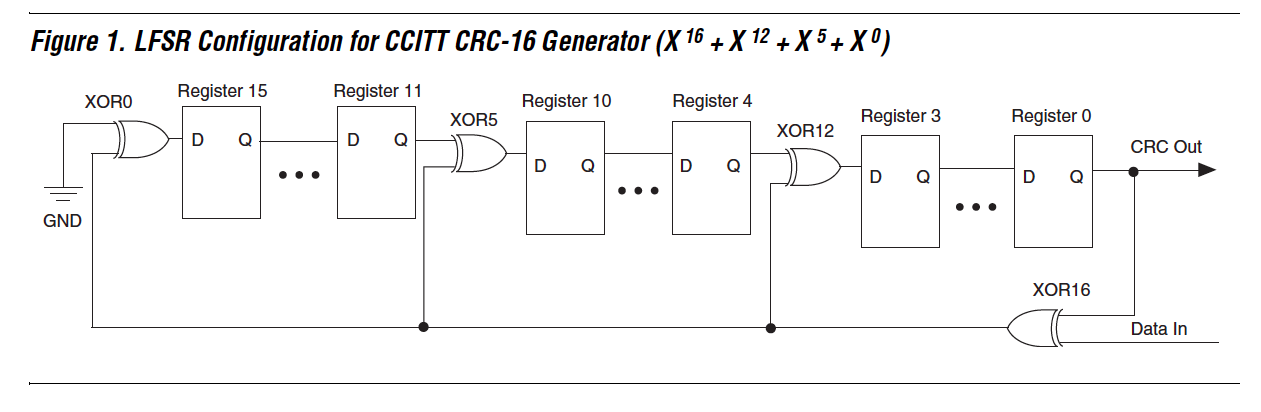
\includegraphics[width=\textwidth]{lfsr.png}
    \end{figure}

\end{frame}

\section{Data input to FPGA}

\begin{frame}{Data input to FPGA}

\begin{itemize}
    \item arduino reads data from raspi initially and is sent to fpga sequentially
    \item output parity bits are colleted from fpga and appended to the end of the input binary signal
    \item same algorithm is implemented to detect the errors in the received signal where crc is zero if no error is occured during the transmission
    \item the error detection can be shown on an arduino serial monitor after collecting the data from the lfsr
\end{itemize}

\end{frame}

\end{document}
